\author{Brown, Daniel}



%---------------------------------------
%---------------Header------------------
%---------------------------------------
\documentclass[
	pdftex,
	fontsize=12pt,          % Schriftgroesse
	DIV10,                  % Angabe bzgl Bestimmung der Seitenabstaende
	ngerman,                % fuer Umlaute, Silbentrennung etc.
	paper=a4,               % Papierformat
	twoside=false,          % einseitiges Dokument
	titlepage,              % es wird eine Titelseite verwendet
	parskip=half,           % Abstand zwischen Absaetzen (halbe Zeile)
	headings=normal,        % Groesse der Ueberschriften verkleinern
	listof=nochaptergap,  % Verzeichnisse im Inhaltsverzeichnis auffuehren.
	bibliography=totoc, % Literaturverzeichnis im Inhaltsverzeichnis auffuehren
	index=totoc,            % Index im Inhaltsverzeichnis auffuehren
	captions=tableheading,  % Beschriftung von Tabellen oberhalb ausgeben
	final                 % Status des Dokuments (final/draft)
]{scrreprt}
\usepackage{scrhack}
% Zeilenabstand
\usepackage[onehalfspacing]{setspace}
% Tabellen
\usepackage{array}
\usepackage{tabularx}
\usepackage{supertabular}
\usepackage{longtable}
\usepackage{hhline}
\usepackage{multirow}
% Grafiken
\usepackage{graphicx}
\usepackage{wrapfig}
\usepackage[svgnames,table,dvipsnames]{xcolor}
\usepackage{floatflt}
\usepackage{float}
% Sprache und Anführungszeichen
\usepackage[T1]{fontenc}
\usepackage[utf8]{inputenc}
\usepackage[ngerman]{babel}
\usepackage{hyphenat}
\usepackage{courier}
\usepackage{palatino}
\usepackage[babel,german=quotes]{csquotes}
\usepackage{eurosym}
% Abstände
\usepackage[margin=25mm,includefoot]{geometry}
% Pakete um Textteile drehen zu können, oder eine Seite Querformat anzeigen kann.
\usepackage{rotating}
\usepackage{lscape}
\usepackage{pdflscape}
\usepackage{enumerate}
% Hurenkinder und Schusterjungen verhindern (http://projekte.dante.de/DanteFAQ/Silbentrennung)
\clubpenalty=10000
\widowpenalty=10000
\displaywidowpenalty=10000
% Fussnoten
\usepackage[hang, multiple, stable]{footmisc}
\usepackage{chngcntr}
\counterwithout{figure}{chapter} 
\counterwithout{equation}{chapter}
\counterwithout{footnote}{chapter}
\counterwithout{table}{chapter}
% Verweise
\usepackage[colorlinks,linkcolor=blue]{hyperref}
\usepackage[nameinlink]{cleveref}
\usepackage[all]{hypcap}
% Verzeichnisse
\usepackage{tocloft}
\tocloftpagestyle{scrheadings}
% Abkürzungsverzeichnis
\usepackage[printonlyused]{acronym}
% Kopfzeile
\usepackage[
automark,     % Kapitelangaben in Kopfzeile automatisch erstellen
headsepline,  % Trennlinie unter Kopfzeile
ilines        % Trennlinie linksbndig ausrichten
]{scrpage2}
% Kopf- und Fusszeilenstil
\pagestyle{scrheadings}
% Kopf- und Fusszeile auch auf Kapitelanfangsseiten
\renewcommand*{\chapterpagestyle}{scrheadings}
% Schriftform der Kopfzeile
\renewcommand{\headfont}{\normalfont}
% Kopfzeile
\ihead{\headmark}
\chead{\hspace{1mm}}
\ohead{Seite \thepage}
\setlength{\headheight}{21mm} % Höhe der Kopfzeile
\setheadsepline[text]{0.4pt} % Trennlinie unter Kopfzeile
% Fusszeile
\cfoot{\hspace{1mm}}
% Namen der Komponenten formatieren
\newcommand{\appref}[1]{\hyperref[app:#1]{\MakeUppercase{#1}}}
% besserer Blocksatz
\sloppy
% externe PDFs einbinden
\usepackage{pdfpages}
% Markierungsfarben der Autoren
\usepackage{soul}
\newcommand{\hlc}[2][yellow]{{\sethlcolor{#1}\hl{#2}}}
\newcommand{\daniel}[1]{\hlc[cyan]{#1}}
\newcommand{\jani}[1]{\hlc[green]{#1}}
\newcommand{\samuel}[1]{\hlc[yellow]{#1}}


%---------------------------------------
%---------------Dokument----------------
%---------------------------------------
\begin{document}
\selectlanguage{ngerman}
\setlength{\parindent}{0mm}
%mindestens 3 Zeilen auf der Seite
\widowpenalties 3 10000 10000 100
\clubpenalties 3 10000 10000 100



%---------------------------------------
%-------------Deckblatt-----------------
%---------------------------------------

\newgeometry{margin=25mm}
\begin{titlepage}	
	\begin{center}
		% Logos der Firma und DHBW
		% 		\vspace*{0cm}
		
\includegraphics[height=2.9cm]{bilder/securitysquad}
		\hfill
		
\includegraphics[height=2.9cm]{bilder/dhbw-logo}	\\ [1.2cm]
		%Titel, Typ der Arbeit, Studiengang
		{\LARGE \textbf{A Walk on the Web’s Wild Side}}	\\ [1cm]
		{\Large  \scshape Projektdokumentation}	\\ [1.2cm]
		{\large für die Vorlesung}	\\ [0.5cm]
		{\large \textbf{angewandtes Projektmanagement}}	\\[0.5cm]
		{\large des Studiengangs Informatik \linebreak Studienrichtung Angewandte Informatik}	\\[0.5cm]
		{\large an der}	\\[0.5cm]
		{\large Dualen Hochschule Baden-Württemberg Karlsruhe}	\\[0.7cm]
		{\large von} 	\\ [0.5cm]
		%Autor und Abgabedatum
		{\large \bfseries \textbf{Daniel Brown}}	\\ [0.8cm]
		{Abgabedatum 22. Mai 2017}
		\vfill
	\end{center}
	\begin{tabular}{l@{\hspace{2cm}}l}
		\textbf{Bearbeitungszeitraum}		& 12 Wochen	\\
		\textbf{Matrikelnummer}				& 3788021	\\
		\textbf{Kurs}						& TINF14B2	\\
		\textbf{Betreuer der Studienarbeit}	& Dr. Martin Johns	\\
		\textbf{Betreuer der Dokumentation}	& Michael Vetter	\\
	\end{tabular}
\end{titlepage}
\restoregeometry



% römische Seitenzahlen
\renewcommand{\thepage}{\Roman{page}}
\setcounter{page}{1}



%---------------------------------------
%-------------Erklärung-----------------
%---------------------------------------
\chapter*{Erklärung}
\markboth{Erklärung}{Erklärung}

\vspace*{2em}

(gemäß §5(3) der \enquote{Studien- und Prüfungsordnung DHBW Technik} vom 29.9.2015)

Ich versichere hiermit, dass ich diese Ausarbeitung selbstständig verfasst habe.

\vspace{3em}
\begin{tabular}{lp{2em}l}
	Karlsruhe, den 22. Mai 2017	&& \textit{Daniel Brown}\hspace{4cm} \\\cline{1-1}\cline{3-3}
	Ort, Datum     				&& Name
\end{tabular}
\newpage



% Verzeichnisse
\tableofcontents
\newpage
\phantomsection
\addcontentsline{toc}{chapter}{Abbildungsverzeichnis}
\listoffigures
\newpage
\phantomsection
\addcontentsline{toc}{chapter}{Tabellenverzeichnis}
\listoftables
\newpage
\phantomsection
\newpage
% --> Seitenzahl speichern für Anhang
\newcounter{SeitenzahlSpeicher}
\setcounter{SeitenzahlSpeicher}{\value{page}}
\newpage
% arabische Nummerierung
\renewcommand{\thepage}{\arabic{page}}
\setcounter{page}{1}



%---------------------------------------
%----------------Inhalt-----------------
%---------------------------------------
\chapter{Randbedingungen dieser Ausarbeitung}

In dieser Arbeit werden alle Projektmanagement-relevanten Aspekte eines Softwareentwicklungsprojektes im Rahmen einer Studienarbeit beschrieben. Die Dokumentation wird zur Leistungsmessung der Vorlesung \textit{angewandtes Projektmanagement} angefertigt und von Michael Vetter betreut.
Da diese Vorlesung im sechsten Semester besucht wird, liegt der Fokus der Ausarbeitung auf der zweiten Hälfte des Projekts.


\newpage
\chapter{Projektdefinition}

Dieses Kapitel beschreibt zunächst die Rahmenbedingungen des Projekts. Danach wird auf das Ziel sowie auf das Projektteam und dessen Lösungsansatz eingegangen.

\section{Rahmenbedingungen}

Der Name der Studienarbeit lautet \textit{A Walk on the Web's Wild Side}. Es findet im Rahmen eines dualen Studiums an der DHBW Karlsruhe statt. Es wird über die Theoriephasen des fünften und sechsten Semesters durchgeführt, wobei dazwischen eine Praxisphase im ausbildenden Betrieb der Studenten stattfindet. Die Dauer des Projekts beträgt somit sechs Monate. Es werden offiziell für jedes Semester 150 Stunden Regelarbeitsaufwand vorgesehen. Bei dem Projekt handelt es sich um ein Softwareentwicklungsprojekt, in dem eine Webanwendung konzipiert und umgesetzt wird.


\section{Problemstellung}

Durchschnittliche Nutzer sind heutzutage im World Wide Web ein gefragtes Angriffsziel für webbasierte Angriffe. Häufig wird hierfür der Nutzer auf maliziöse Webseiten gelockt. Diese Webseiten nutzen dann unter anderem Sicherheitslücken im Browser des Nutzers um Schadsoftware zu verbreiten oder den Anwender auszuspähen. Die Studienarbeit beschäftigt sich mit diesen Webseiten und analysiert deren Bedrohungspotenzial.

\section{Projektziel}
Ziel des Projekts ist eine systematische Untersuchung der Aktivitäten von semi-legalen Webseiten im World Wide Web. Das erwartete Ergebnis ist ein Prüfportal, auf dem jene Webseiten automatisiert analysiert und Ergebnisse präsentiert werden sollen. Nach dem Erstellen einer Übersicht von interessanten Zielen, wie z.B. One-Click-Hoster oder File-sharing Seiten sollen ausgewählte Webseiten manuell untersucht werden. Außerdem sollen verschiedene Angriffsszenarien zur weiteren Prüfung ausgewählt werden. Der Untersuchungsprozess der Webseiten soll im Verlauf der Arbeit stückweise automatisiert und in den Rahmen einer Prüfanwendung gebracht werden. Abschließend sollen eine Vielzahl von Webseiten mit der Anwendung getestet und die Ergebnisse ausgewertet und dokumentiert werden.

\section{Anforderungen}
Durch die Aufgabenstellung und das Erstgespräch ergeben sich folgende Anforderungen:
\begin{description}
	\item[Prüfung auf clientseitiger Angriffe]{bestimmte Webseiten sollen auf sicherheitsrelevante Schwachstellen und clientseitige Angriffe überprüft werden können.}
	\item[Tests in gesichertem Umfeld]{Die Sicherheitstests müssen abgeschottet vom Hauptsystem laufen, um vor Schadware und clientseitige Angriffe zu sein.}
	\item[Benutzerfreundliche Oberfläche]{Die Anwendung muss von Durchschnittsnutzern benutzbar sein. Es sollen keine komplexen Formulare ausgefüllt und konfiguriert werden.}
	\item[Tests in gesichertem Umfeld]{Die Sicherheitstests müssen abgeschottet vom Hauptsystem laufen, um vor Schadware und clientseitige Angriffe zu sein.}
	\item[Automatische Überprüfung]{Die Durchführung der Sicherheitstests soll voll automatisch erfolgen.}
	\item[Darstellbarkeit der Ergebnisse]{Die Ergebnisse der Analysephase sollen zur Dokumentation einsehbar sein.}
\end{description}


\section{Team und Zuständigkeiten}

Das Entwicklerteam besteht aus drei Studenten der angewandten Informatik: Samuel Philipp, Daniel Brown und Jan-Eric Gaidusch. Daniel Brown ist für das Projektmanagement verantwortlich, Jan-Eric Gaidusch für die Testdurchläufe in der virtualisierten Umgebung und Samuel Philipp für das Frontend. Der Verantwortliche ist nicht zwingend der Umsetzende, sondern lediglich erster Ansprechpartner. Der Name der Arbeitsgruppe ist SecuritySquad\footnote{Der Name \textit{SecuritySquad} ist angelehnt an den Titel des US-amerikanischen Actionfilms SuicideSquad.}. Eine genauere Beschreibung der Arbeitsgruppe kann auf der Webseite \url{https://www.securitysquad.de} eingesehen werden. \Cref{fig:securitysquad-logo} zeigt das Logo des Teams.

\begin{figure}[H]
	\centering
	
\includegraphics[width=5cm]{bilder/securitysquad}
	\caption{\textit{SecuritySquad} - Logo}
	\label{fig:securitysquad-logo}
\end{figure}

Die Studienarbeit wird von Dr. Martin Johns betreut, der an der DHBW Karlsruhe die
Vorlesung Datensicherheit hält. Hauptberuflich ist er Forscher eben dieses Gebietes am
CEC Karlsruhe der SAP SE. 3


\section{Vision}

\textit{webifier} ist eine Anwendung mit der Webseiten auf deren Seriosität und mögliche clientseitige Angriffe auf den Nutzer geprüft werden können. Sie besteht aus mehreren eigenständigen Teilanwendungen. Im Zentrum steht der Tester, welcher die einzelnen Tests verwaltet, ausführt und anschließend die Ergebnisse auswertet. Jeder einzelne Test ist eine weitere isolierte Teilanwendung des Testers. So kann jeder Test unabhängig
von allen anderen betrieben werden.

\begin{figure}[H]
	\centering
	
\includegraphics[width=5cm]{bilder/webifier}
	\caption{\textit{webifier} - Logo}
	\label{fig:webifier-logo}
\end{figure}

\textit{webifier} Plattform ist eine Webanwendung welche den Endnutzern eine grafische Oberfläche zur Verfügung stellt, um Webseiten zu überprüfen. Im Hintergrund nutzt die
Plattform den Tester. \textit{webifier} Mail ist ein Dienst mit dem Links aus E-Mails überprüft werden können. Anschließend erhält der Sender eine E-Mail mit den Resultaten zurück. Eine weitere Teilanwendung ist \textit{webifier} Data. Sie stellt eine Schnittstelle für den Tester bereit, um alle Testergebnisse sammeln zu können. \textit{webifier} Statistics ist die letzte Teilanwendung von \textit{webifier}. Sie nutzt die vom Data-Modul gespeicherten Daten um Auswertungen aller Testergebnisse bereitzustellen.


\newpage
\chapter{Projektplanung}


\section{Terminplan}

In diesem Abschnitt werden alle Phasen, Meilensteine und deren Termine tabellarisch in \Cref{tab:terminplan} aufgelistet.

\begin{table}[H]
\begin{tabular}[H]{|l|c|c|c|}
	\hline
	\rowcolor{lightgray}\textbf{Name} & \textbf{Beteiligte} & \textbf{Startdatum} & \textbf{Enddatum} \\\hline
	Umsetzungsphase & Team & 13.02.2016 & 26.03.2016 \\\hline
	Startgespräch Semester 6 & alle & \multicolumn{2}{c|}{06.03.2017} \\\hline
	Besprechung der schriftlichen Arbeit & alle & \multicolumn{2}{c|}{03.04.2017} \\\hline
	Analysephase & Team & 27.03.2016 & 26.04.2016 \\\hline
	Vorstellung der Analyseergebnisse & alle & \multicolumn{2}{c|}{24.04.2017} \\\hline
	Abschlussgespräch & alle & \multicolumn{2}{c|}{03.05.2017} \\\hline
	Fertigstellung der Studienarbeit & Team & \multicolumn{2}{c|}{05.05.2017} \\\hline
	Präsentation der Studienarbeit & Team & \multicolumn{2}{c|}{12.05.2017} \\\hline
	Gegenlesen der Studienarbeit & alle & 05.05.2017 & 10.05.2017 \\\hline
	Abgabe der Studienarbeit & Team & \multicolumn{2}{c|}{15.05.2017} \\\hline
\end{tabular}
	\caption{Terminplan}
	\label{tab:terminplan}
\end{table}

\section{Risikomanagement}

\Cref{tab:risiken} listet Risiken auf. Zusätzlich gibt sie deren Auswirkungsgrad, Wahrscheinlichkeit und mögliche Maßnahmen an. Harmlose Risiken werden in \textcolor{green}{grün} dargestellt, gefährliche in \textcolor{yellow}{gelb} und fatale in \textcolor{RedOrange}{rot}

\begin{table}[H]
\begin{tabular}{|p{3cm}|c|p{3cm}|p{5cm}|}
	\hline
	\rowcolor{lightgray}\textbf{Risiko} & \textbf{Auswirkung} & \textbf{Wahrschein-lichkeit} & \textbf{Prävention \& Schadensbegrenzung} \\\hline
	\rowcolor{green}Virtualisierungstechnik nicht sicher genug & hoch & gering & - \\\hline
	\rowcolor{yellow}fehlendes Know-How & hoch & mittel & gutes Konzept, Betreuer fragen \\\hline
	\rowcolor{yellow}Krankheit & mittel & mittel & Krankheit in Zeitplanung mit einplanen \\\hline
	\rowcolor{red}Missverständnisse mit Betreuer & mittel & hoch & regelmäßiger Austausch und Demos \\\hline
	\rowcolor{red}Serverleistung zu gering & hoch & mittel & Upgrade oder Angebotswechsel \\\hline
	\rowcolor{red}Zeitmangel des Teams & hoch & hoch & Prüfungsphase in Zeitplanung mit einplanen, Zusatzfeatures weglassen \\\hline
\end{tabular}
	\caption{Risiken}
	\label{tab:risiken}
\end{table}


\section{Arbeitsmittel}

Für die Entwicklung der Anwendung und das Schreiben der Studienarbeit wurden folgende Werkzeuge und Hilfsmittel verwendet:
\begin{description}
	\item[Laptop] Jedes Teammitglied besitzt einen Laptop um die Anwendung zu entwickeln und die Studienarbeit auszuarbeiten. Diese wurden privat beschafft.
	\item[Entwicklungsumgebung] Jedes Teammitglied besitzt eine Programm auf dem Laptop, mit dem die Anwendung umgesetzt wird. Alle drei Mitglieder verwenden \textit{IntelliJ IDEA} als Entwicklungsumgebung. Da es sich bei den Entwicklern um Studenten handelt, kann die Software kostenlos heruntergeladen und installiert werden.
	\item[LaTeX-Editor] Die Arbeit wird in LaTeX geschrieben. Deshalb hat jedes Teammitglied ein Programm zur erleichterten Erstellung von Texten in ebendieser Sprache. Es werden die kostenlosen Tools \textit{TeXclipse}, \textit{Texmaker} und \textit{TeXstudio} verwendet. Alle drei sind kostenlos nutzbar.
	\item[einfacher Root-Server] Dieser wird von der Firma \textit{netcup} für 12 Monate angemietet. Die Gebühren für den Server werden von der DHBW erstattet.
	\item[leistungsstarker Root-Server] Dieser Server wird ebenfalls von der Firma \textit{netcup} gestellt. Allerdings wird dieser nur für einen Monat gebucht, da er nur für die Analysephase gebraucht wird.
	\item[GitHub] Für Versionskontrolle und Zusammenarbeit der Entwicklung und der wissenschaftlichen Arbeit wird die Plattform GitHub genutzt. Sie ist kostenlos und in die Entwicklungsumgebung integriert.
	\item[Google Drive \& Google Docs] Für Versionskontrolle in Dokumentation und Organisation wird der File-Sharing Dienst \textit{Google Drive} genutzt. Um gemeinsam an einem Dokument zu arbeiten wird die Webanwendung \textit{Google Docs} verwendet. Beide Hilfsmittel sind kostenlos, können aber in der regel nur über einen Browser verwendet werden.
	\item[Slack] Um miteinander zu kommunizieren wird der Chatservice \textit{Slack} genutzt. Dieser ist ebenfalls kostenlos und bietet Integrationsmöglichkeiten für \textit{GitHub} und \textit{Google Drive} an.
	\item[Google Hangouts] Meetings, die nicht persönlich abgehalten werden können, werden über \textit{Google Hangouts} gehalten. Dabei handelt es sich um eine Webanwendung, hauptsächlich für Audio- und Videokonferenzen genutzt wird. Es bietet zusätzlich die Möglichkeit, seinen Bildschirm zu übertragen.
\end{description}



\newpage
\chapter{Projektdurchführung}

Die Entwicklung der Webanwendung wird in der wissenschaftlichen Arbeit beschrieben, die im Rahmen des Projekts erstellt wurde. Diese kann im Internet auf \url{https://github.com/SecuritySquad/Studienarbeit/releases/download/abgabe/Studienarbeit.pdf} eingesehen werden.


\section{Schreiben der Studienarbeit}

Zur Anfertigung der Studienarbeit wird zunächst eine Gliederung erstellt. Jedes Teammitglied bekommt gleich viele Kapitel bzw. Abschnitte zugeteilt. Dabei wird darauf geachtet, dass die zu schreibenden Texte in Summe für alle etwa gleich lang sind und dass jeder einen etwa gleichen Anteil an Einleitung, Grundlagen, Konzept, Umsetzung, Analyse und Fazit hat.

Zu beginn des zweiten Semesters sind lediglich einige Teile der Grundlagen fertig ausformuliert. Dies liegt daran, dass hauptsächlich an der Umsetzung der Anwendung sowie deren Zusatzfeatures gearbeitet wird. Es gibt keine festen Meilensteine für die Kapitel der Studienarbeit, sodass nicht auf eine mittelfristige Deadline hingearbeitet wird. Neben den regelmäßigen Videokonferenzen im Team und den Meetings mit dem Betreuer gibt es lediglich entwicklungsbezogene Meilensteine und Phasentermine.

Einen Monat vor Abgabe beginnt das Team deshalb konzentriert an der wissenschaftlichen Arbeit zu schreiben. Die Studienarbeit ist in sieben Kapitel unterteilt. Das erste Kapitel ist die Einleitung. Hier werden die Rahmenbedingungen für die Arbeit erläutert und es wird ein Einblick in die Hintergründe gegeben. Das nächste Kapitel, Grundlagen, behandelt Tools, die maßgeblich zur Entwicklung der Lösung verwendet werden. Weiterhin werden clientseitige Probleme bzw. Angriffspunkte fachlich aufbereitet, die in der Lösung angesprochen werden. Im dritten Kapitel werden die Ergebnisse des Entwurfsprozesses dargestellt und begründet. Dabei wird grundsätzlich zwischen der Gesamtanwendung und den Tests unterschieden. Diese Aufteilung findet sich auch im darauffolgenden Kapitel, der Umsetzung, wieder. Dort wird hingegen auf die konkrete Implementierung des Konzepts eingegangen und bedeutende Anwendungslogik anhand von Codebeispielen erklärt. In Kapitel fünf, der Analyse, werden die Erkenntnisse der Arbeit präsentiert und danach beurteilt. Zum Abschluss der Arbeit werden in Ausblick und Fazit Ideen und Verbesserungsvorschläge für mögliche Folgeprojekte vorgetragen und die Arbeit abschließend bewertet.


\section{Probleme}
Jedes Mal, wenn ein Mitglied einen Abschnitt fertigstellt, veröffentlicht es seine Änderungen auf die Plattform \textit{GitHub} über den Befehl \texttt{git push}. Dies funktioniert jedoch nicht immer, denn wenn in der Zwischenzeit ein anderer seine Änderungen veröffentlicht hat, dann müssen diese Änderungen zunächst auf die eigene Version angewandt werden. Dies geht im besten Fall über den Befehl \texttt{git pull}. Dabei werden alle reinkommenden Änderungen über einen Algorithmus eingepflegt. Schlägt der Algorithmus in einer Datei fehl, müssen die Änderungen auf die Datei manuell eingepflegt werden. Dieser Vorgang wird als \textit{merge} bezeichnet und kann bei großen Änderungen sehr Zeitintensiv sein. Er wird über den Befehl \texttt{git merge} eingeleitet. Sind alle Änderungen übernommen, so kann die eigene Version des Projektes veröffentlicht werden.

Zudem gibt es Probleme beim kompilieren des Projektes. Nicht jeder benutzt die gleiche LaTeX-Distribution und Version, was dazu führt, dass das Projekt nicht auf jedem Entwicklerlaptop gebaut werden kann.

Am 05.04.2017 um 10:42 Uhr trifft aus heiterem Himmel eine Hinweismail des Serverproviders \textit{netcup} ein. Der Mailverkehr zu diesem Thema ist in \Cref{mail:abuse} zu finden. Das \textit{Bundesamt für Sicherheit in der Informationstechnik} (BSI) habe Zugriffe auf einen ihrer \textit{Honeypots} erkannt und den Server als \textit{gekaperten Rechner} eingestuft. Dies ist nicht verwunderlich, da es das Ziel unserer Sicherheitstest ist, maliziöse Webseiten zu untersuchen. Wenn diese Seiten vom BSI übernommen werden und diese sich dann melden, ist kann dies als Zeichen des Erfolgs gesehen werden. Auch wenn der Schock zunächst Tief sitzt, muss schnell gehandelt werden. Denn ohne eine rasche Antwort würde der Server abgeschaltet werden. Aus diesem Grund wird ein Anruf bei \textit{netcup} getätigt und die Lage geschildert. Der Server ist enorm sicher vor Angriffen, da die Anwendung so aufgebaut ist, dass der einzige Kontakt mit den zu testenden Webseiten nur in abgeschotteten, virtuellen Umgebungen stattfindet. Nach diesem Gespräch wird der Server wieder als \textit{unbedenklich} eingestuft und die Analysephase kann wie geplant fortgesetzt werden.

Die Analysephase geht länger als geplant, da der leistungsstarke Server ab und zu abstürzt und das System neu aufgesetzt werden muss. Glücklicherweise ist die Datenbank separat gespeichert, sodass bereits gespeicherte Testergebnisse nicht verloren gehen. Zusätzlich beginnt im Mai die Prüfungsphase, sodass das Team sich weniger um das Projekt kümmern kann. Aufgrund dieser Gegebenheiten muss die Fertigstellung der Arbeit weiter nach hinten verschoben werden.

\newpage
\chapter{Qualitätssicherung}
Die folgenden Abschnitte schildern Maßnahmen die zur Sicherung der Qualität geplant und durchgeführt werden. Zunächst aber werden grundsätzliche Maßnahmen aufgelistet:

\begin{description}
	\item[Versionskontrolle in GitHub] Der Code der Anwendung und der Studienarbeit wird auf \textit{GitHub} gesichert, sodass nachverfolgt werden kann, zu welchem Zeitpunkt welcher Code aktuell ist. Zudem ermöglicht es ein einheitliches Zusammenarbeiten im Team.
	\item[Dokumente in Google Drive] Dokumente, die für das Projektmanagement und andere organisatorische Aufgaben wichtig sind, werden in \textit{Google Drive} gespeichert. Dokumente können über \textit{Google Docs} von mehreren Benutzern gleichzeitig, online und live bearbeitet werden. Zusätzlich ermöglicht es eine beschränkte Versionskontrolle aller Dokumente.
	\item[regelmäßige Meetings mit dem Betreuer] \textit{}
\end{description}

\section{Entwicklung der Anwendung}
Zur Qualitätssicherung der Software werden folgende Maßnahmen ergriffen:

\begin{description}
	\item[Einheitliches Ergebnisschema] Alle Tests müssen eine Antwort liefern, die in das Schema der Hauptanwendung pass. Die Struktur ist fest vorgegeben und wird bei jedem Testdurchlauf geprüft.
	\item[Code Reviews] Bei kritischen Codestellen werden \textit{Code Reviews} durchgeführt. Dabei wird der Code vom jeweiligen Entwickler mindestens einem anderen Teammitglied erklärt. Das Review wird über \textit{Google Hangouts} gemacht, wobei darüber auch der Bildschirm übertragen wird.
	\item[Pair Programming] Bei zentralen Codestellen, oder wenn ein Entwickler Unterstützung benötigt, wird zusammen im \textit{Pair Programming} entwickelt. Dazu holt er sich mindestens einen weiteren Entwickler zur Hilfe und startet seine Videokonferenz in \textit{Google Hangouts}. Nun übernimmt einer die Rolle des \textit{Schreibers}, der andere wird zum \textit{Denker}. Der \textit{Schreiber} überträgt seinen Bildschirm und lässt sich vom \textit{Denker} den Code diktieren. Nach einer gewissen Zeit werden die Rollen dann getauscht.
\end{description}

\section{Schreiben der Studienarbeit}
Um die Qualität der Studienarbeit sicherzustellen, werden folgende Maßnahmen ergriffen:

\begin{description}
	\item[Abkürzungsverzeichnis]{Um häufig vorkommende Abkürzungen einheitlich zu schreiben, wird ein Abkürzungsverzeichnis angelegt. Die darin enthaltenen Abkürzungen werden per LaTeX-Befehl \texttt{\textbackslash ac\{\textit{ABK}\}} eingebunden und beim Kompilieren überprüft. Zusätzlich gibt es die Möglichkeit für generell häufig verwendete Begriffe ein \textit{Glossar} anzulegen. Da die meisten häufig verwendeten Begriffe jedoch im Kapitel \textit{Grundlagen} beschrieben werden, wird kein \textit{Glossar} verwendet.}
	\item[Vorgaben für die Arbeit]{Alle selbst erdachten, in der Arbeit verwendeten Begriffe werden in einem Dokument namens \textit{Vorgaben Einheit Studienarbeit} eingetragen. Alle Teammitglieder haben sich an die dort festgelegten Konventionen und Schreibweisen zu halten. Dies wird vor Abgabe der Arbeit manuell überprüft. Das Dokument ist in \Cref{pdf:einheit} im Anhang zu finden.}
	\item[Gegenlesen kritischer Abschnitte]{Alle selbst erdachten, in der Arbeit verwendeten Begriffe werden in einem Dokument namens \textit{Vorgaben Einheit Studienarbeit} eingetragen. Alle Teammitglieder haben sich an die dort festgelegten Konventionen und Schreibweisen zu halten. Dies wird vor Abgabe der Arbeit manuell überprüft. Das Dokument ist in \Cref{pdf:einheit} im Anhang zu finden.}
	\item[Kompilierhinweise]{Beim Kompilieren der Arbeit werden Fehler- und Warnhinweise ausgegeben. Fehler müssen völlig beseitigt werden, um überhaupt eine PDF generieren zu können. Warnungen hingegen werden nur teilweise behoben, da darunter auch irrelevante Meldungen wie z.B. \texttt{Underfull \textbackslash hbox (badness 10000) in paragraph} oder \texttt{destination with the same identifier (name{page.1}) has been already used, duplicate ignored} sind.}
	\item[Zuordnung zwischen Autoren und Kapiteln]{Um den Überblick über die Autoren der jeweiligen Kapitel und Abschnitte zu behalten, wird eine Liste der Verantwortlichen erstellt. Diese ist in \Cref{pdf:autoren} abgebildet.}
\end{description}

\newpage
\chapter{Projektabschluss}
Dieses Kapitel beschreibt die Schlussaktivitäten und gibt eine Zusammenfassung des Projekts.

\section{Übergabe}
Nach Fertigstellung der Arbeit wird diese von jedem Teammitglied in Moodle hochgeladen. Die selbe Version wird per E-Mail an den Betreuer zur Bewertung eingereicht. Außerdem werden für jedes Mitglied zwei Druckfassungen erstellt, wobei eine zur Abgabe für das Sekretariat der DHBW und die andere für den persönlichen Gebrauch gedacht sind.

Die Rechte der Entwicklergruppe auf \textit{GitHub} bleiben zunächst im Besitz des Teams. Bei Fortführung des Projekts werden die entsprechenden Studenten aufgenommen. Der Server und somit auch die online Webanwendung wird bis Ende November weiterlaufen. Bei dem Zugriff auf diese verhält es sich wie bei der Entwicklergruppe. Die Berechtigung auf \textit{Google Drive} und \textit{Slack} bleiben ebenfalls wie gehabt.

Ein Backup der Datenbank wird rechtzeitig gesichert und an den Betreuer weitergeleitet. Die bei der Abgabe aktuelle Version der Anwendung \textit{webifier} wird auf \textit{GitHub} gekennzeichnet werden. Über diese Plattform können Interessenten die Software herunterladen und installieren. Mögliche zukünftige Studienarbeiten werden die Entwicklung ab dieser Version fortsetzen.


\section{Erkenntnisse}
Um ein angenehmes und gleichmäßiges Arbeitstempo zu gewährleisten müssen für alle anzufertigenden Artefakte möglichst kleine Meilensteine definiert werden, die nicht länger als einen Monat entfernt liegen sollten. Dies hätte den Verzug der Abgabe der Studienarbeit wesentlich gemindert bzw. ganz verhindert.

Regelmäßige Treffen mit Stakeholdern (vor allem Auftraggebern) helfen dabei, das Projekt nicht in eine falsche Richtung laufen zu lassen. Dabei sollten die erreichten Ergebnisse nicht nur theoretisch durchgesprochen werden, sondern auch möglichst praktisch gezeigt werden. Dies lässt sich bei Software am besten durch eine Demo bewerkstelligen.





% römische Nummerierung --> SeitenzahlSpeicher
\newpage
\stepcounter{SeitenzahlSpeicher}
\renewcommand{\thepage}{\Roman{page}}
\setcounter{page}{\theSeitenzahlSpeicher}



%---------------------------------------
%---------------Anhang------------------
%---------------------------------------
\appendix
\chapter{Dokumente}

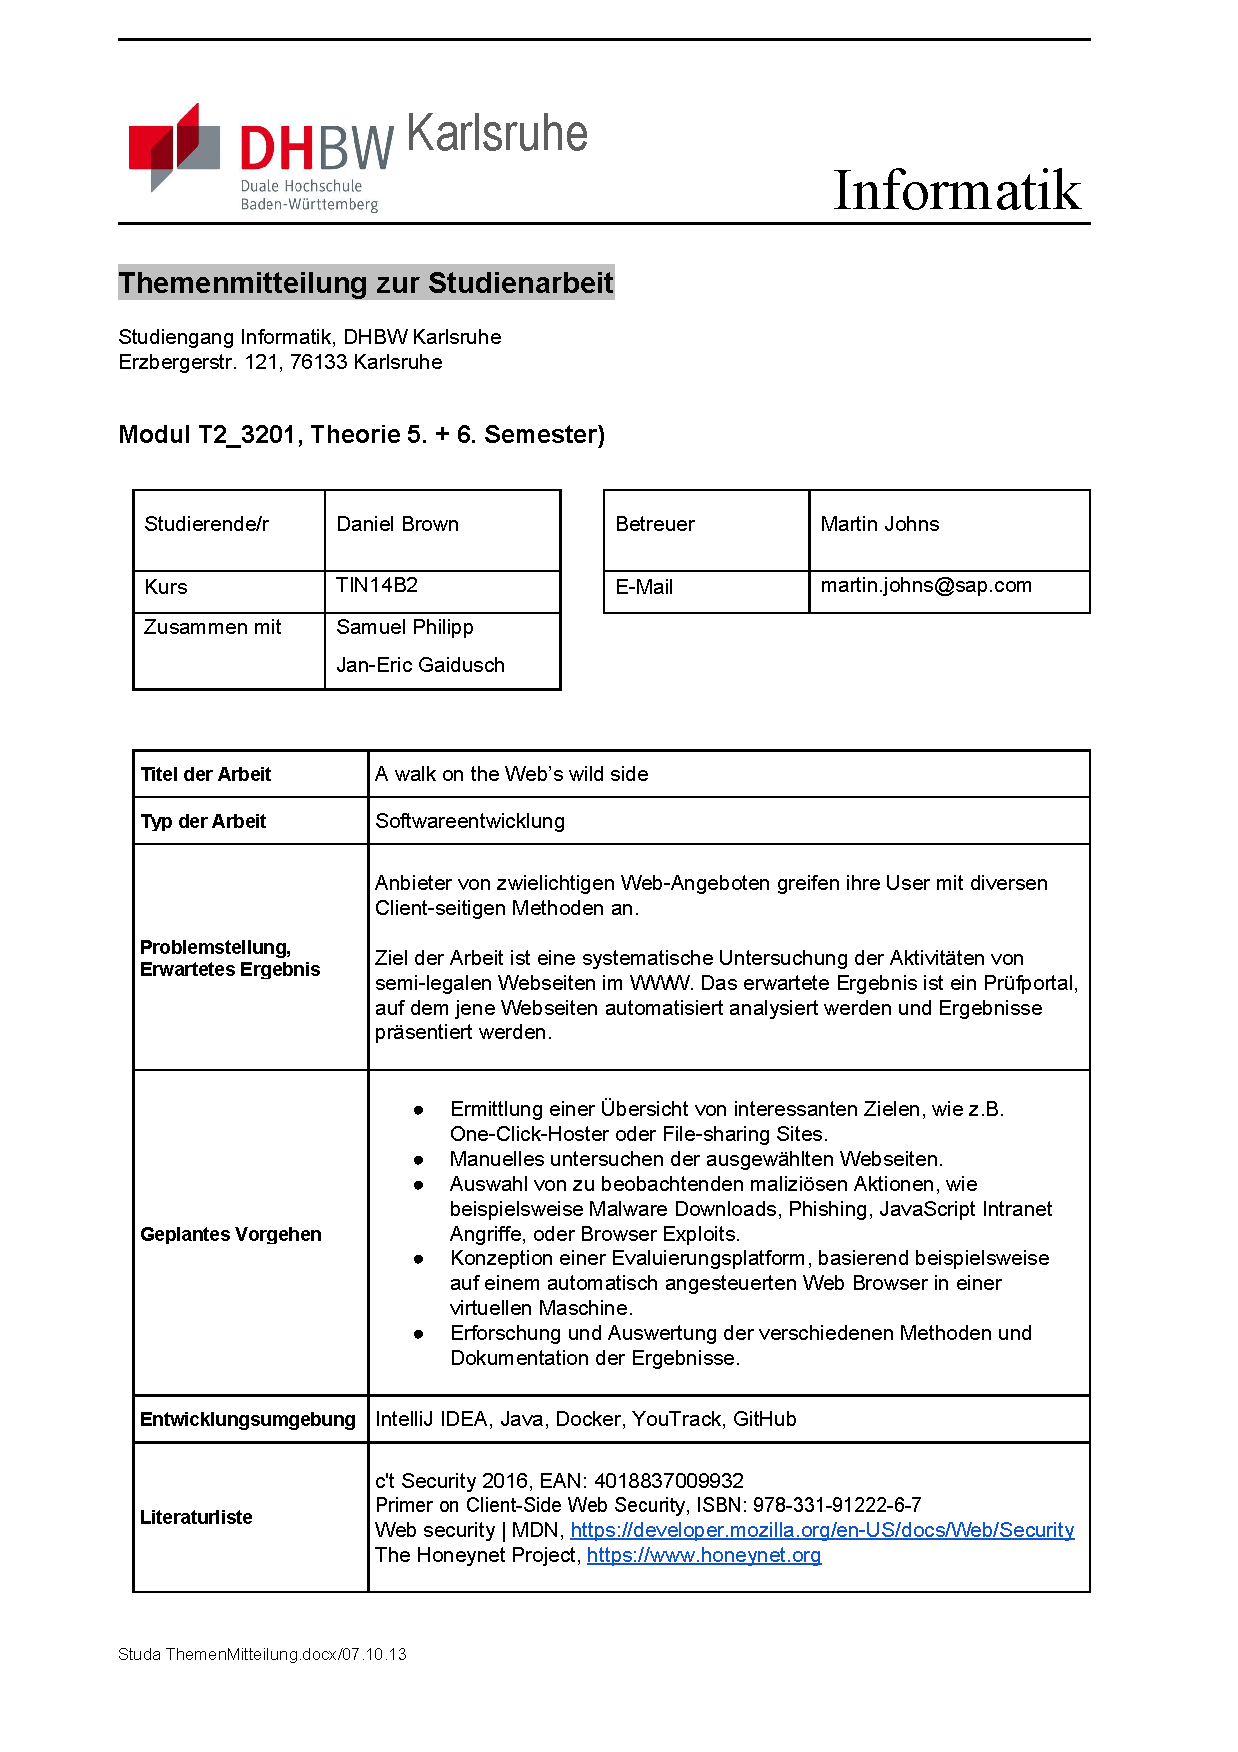
\includepdf[scale=0.8,pages=1,pagecommand=\section{Themenmitteilung zur Studienarbeit}\label{pdf:thema}]{pdfs/thema.pdf}

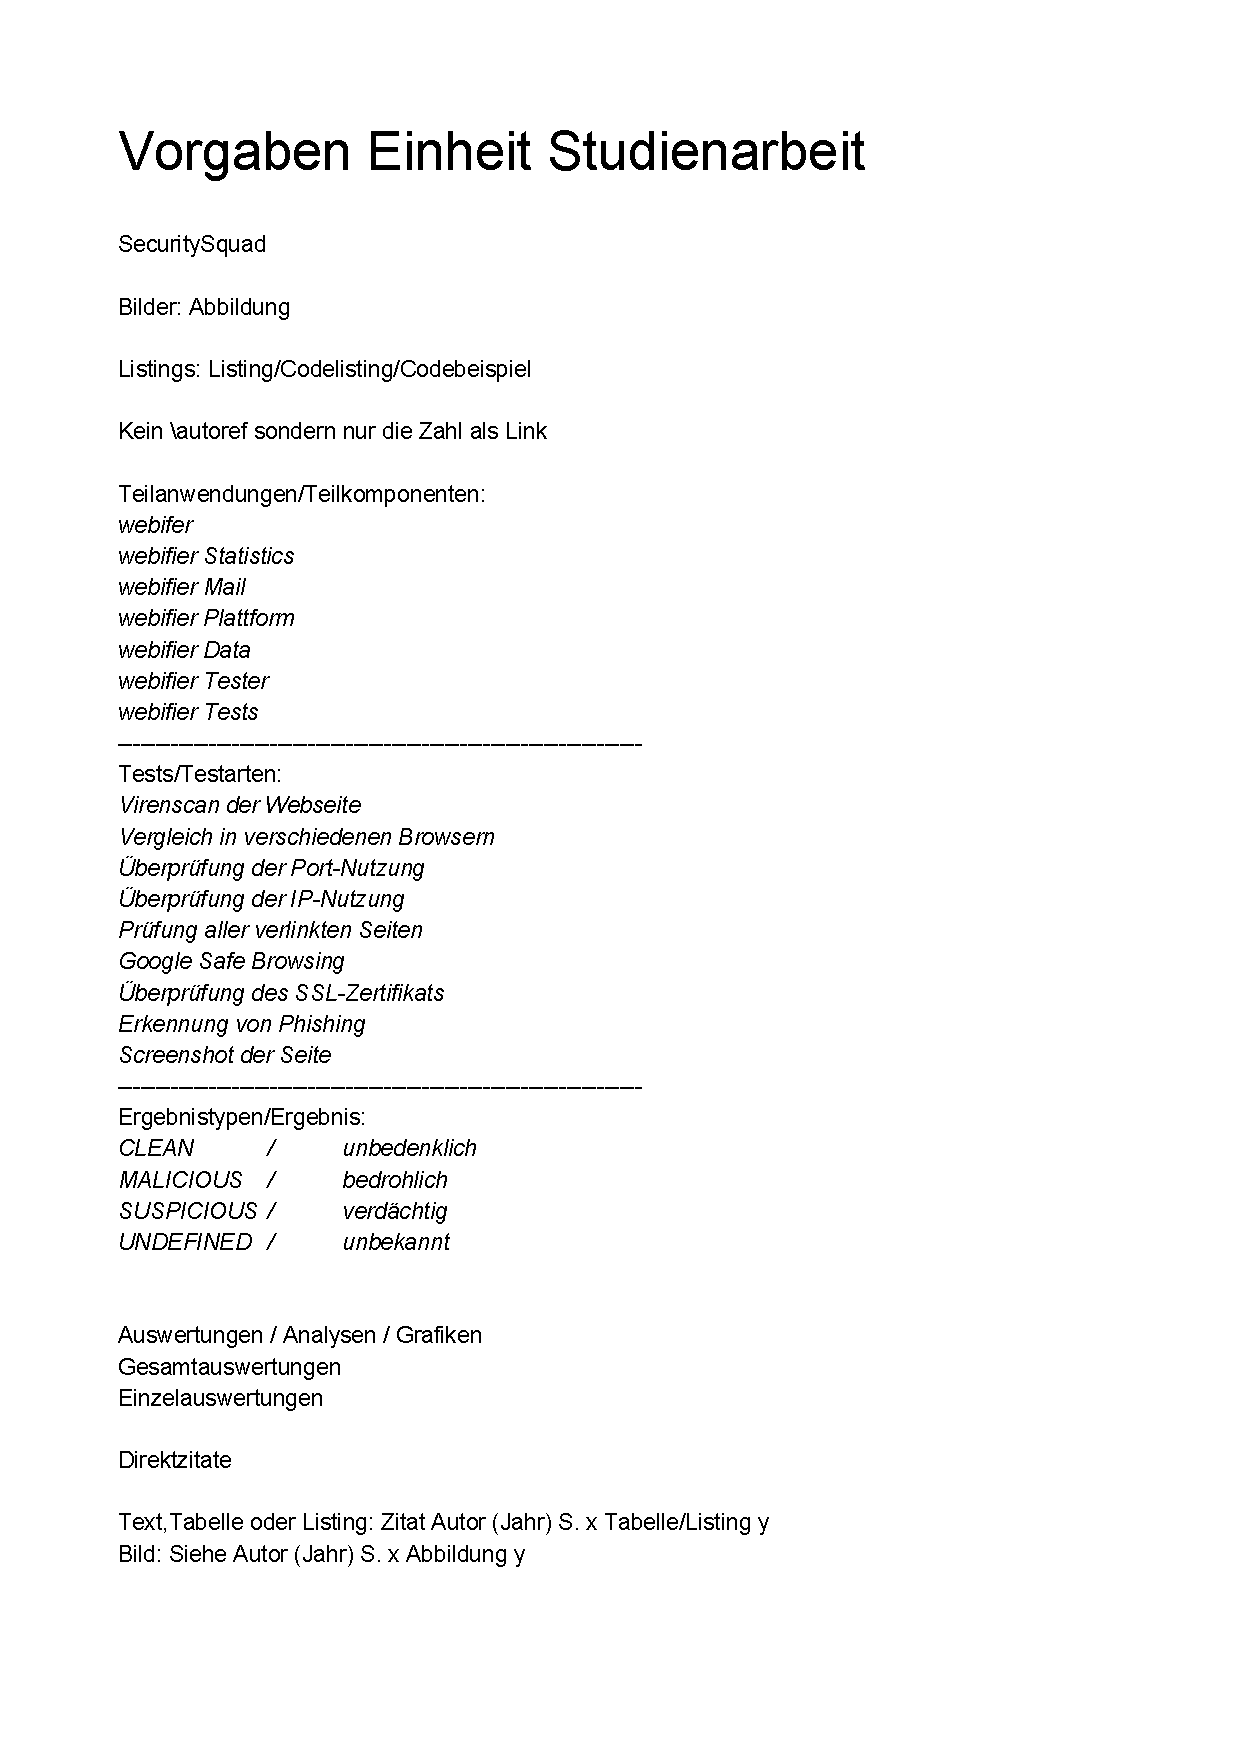
\includepdf[scale=0.8,pages=1,pagecommand=\section{Vorgaben Einheit Studienarbeit}\label{pdf:einheit}]{pdfs/einheit.pdf}

\section{Autoren der einzelnen Kapitel}
\label{pdf:autoren}
Auf den folgenden Seiten werden die Kapitel in den Farben der Autoren markiert.
Dabei steht die Farbe gelb für \samuel{Samuel Philipp}, blau für \daniel{Daniel Brown} und grün für \jani{Jan-Eric Gaidusch}.

\rule{\textwidth}{1pt}

\daniel{Abstract}

\jani{1 Einleitung}

\daniel{1.1 Aufbau der Arbeit}

\samuel{1.2 Aufgabenstellung}

\daniel{1.3 Team}

\samuel{1.4 webifier}

{2 Grundlagen}

{2.1 Frontend Technologien und Framework}

\begin{itemize}
	\item \daniel{HTML}
	\item \daniel{CSS}
	\item \daniel{JavaScript}
	\item \daniel{jQuery}
	\item \daniel{Bootstrap}
\end{itemize}

{2.2 Backend Technologien und Frameworks}

\begin{itemize}
	\item \samuel{Java}
	\item \samuel{Spring}
	\item \samuel{MongoDB}
	\item \jani{Gradle}
	\item \jani{Rest}
	\item \jani{Docker}
	\item \jani{R}
\end{itemize}

{2.3 Technologien und Frameworks der Tests}

\begin{itemize}
	\item \daniel{- Python}
	\item \daniel{- PhantomJS}
	\item \jani{- Bro}
	\item \samuel{- HTtrack}
	\item \samuel{- Resemble.js}
\end{itemize}

\samuel{2.4 Angriffstypen}

\samuel{2.4.1 Malware}

\daniel{2.4.2 Request Header Investigation}

\jani{2.4.3 JavaScript Port \& IP Scanning}

\samuel{2.4.4 Phishing}

{3 Konzept}

\samuel{3.1 }\daniel{Gesamt}\jani{konzept}

\jani{3.1.1 webifier Tests}

\samuel{3.1.2 webifier Tester}

\samuel{3.1.3 webifier Plattform}

\daniel{3.1.4 webifier Mail}

\samuel{3.1.5 webifier Data}

\jani{3.1.6 webifier Statistics}

{3.2 Testarten}

\samuel{3.2.1 Virenscan der Webseite}

\daniel{3.2.2 Vergleich in verschiedenen Browsern}

\jani{3.2.3 \"Uberpr\"ufung der Port-Nutzung}

\jani{3.2.4 \"Uberpr\"ufung der IP-Nutzung}

\daniel{3.2.5 Pr\"ufung aller verlinkten Seiten}

\daniel{3.2.6 Google Safe Browsing}

\samuel{3.2.7 \"Uberpr\"ufung des SSL-Zertifikats}

\samuel{3.2.8 Erkennung von Phishing}

\jani{3.2.9 Screenshot der Seite}

{4 Umsetzung}

\samuel{4.1 }\daniel{Gesamt}\jani{system}

\jani{4.1.1 webifier Tests}

\samuel{4.1.2 webifier Tester}

\samuel{4.1.3 webifier Plattform}

\daniel{4.1.4 webifier Mail}

\samuel{4.1.5 webifier Data}

\jani{4.1.6 webifier Statistics}

{4.2 Tests}

\samuel{4.2.1 Virenscan der Webseite}

\daniel{4.2.2 Vergleich in verschiedenen Browsern}

\jani{4.2.3 \"Uberpr\"ufung der Port-Nutzung}

\jani{4.2.4 \"Uberpr\"ufung der IP-Nutzung}

\daniel{4.2.5 Pr\"ufung aller verlinkten Seiten}

\daniel{4.2.6 Google Safe Browsing}

\samuel{4.2.7 \"Uberpr\"ufung des SSL-Zertifikats}

\samuel{4.2.8 Erkennung von Phishing}

\jani{4.2.9 Screenshot der Seite}

\samuel{5 An}\jani{alyse}

\jani{5.1 Gesamtauswertungen}

\jani{5.2 Einzelauswertungen}

\samuel{5.2.1 Virenscan der Webseite}

\daniel{5.2.2 Vergleich in verschiedenen Browsern}

\jani{5.2.3 \"Uberpr\"ufung der Port-Nutzung}

\jani{5.2.4 \"Uberpr\"ufung der Port-Nutzung}

\daniel{5.2.5 Pr\"ufung aller verlinkten Seiten}

\daniel{5.2.6 Google Safe Browsing}

\samuel{5.2.7 \"Uberpr\"ufung des SSL-Zertifikats}

\samuel{5.2.8 Erkennung von Phishing}

\jani{5.3 Bewertung der Ergebnisse}

\samuel{6 Ausblick}

\samuel{7 Fa}\jani{zit}


\chapter{E-Mails}

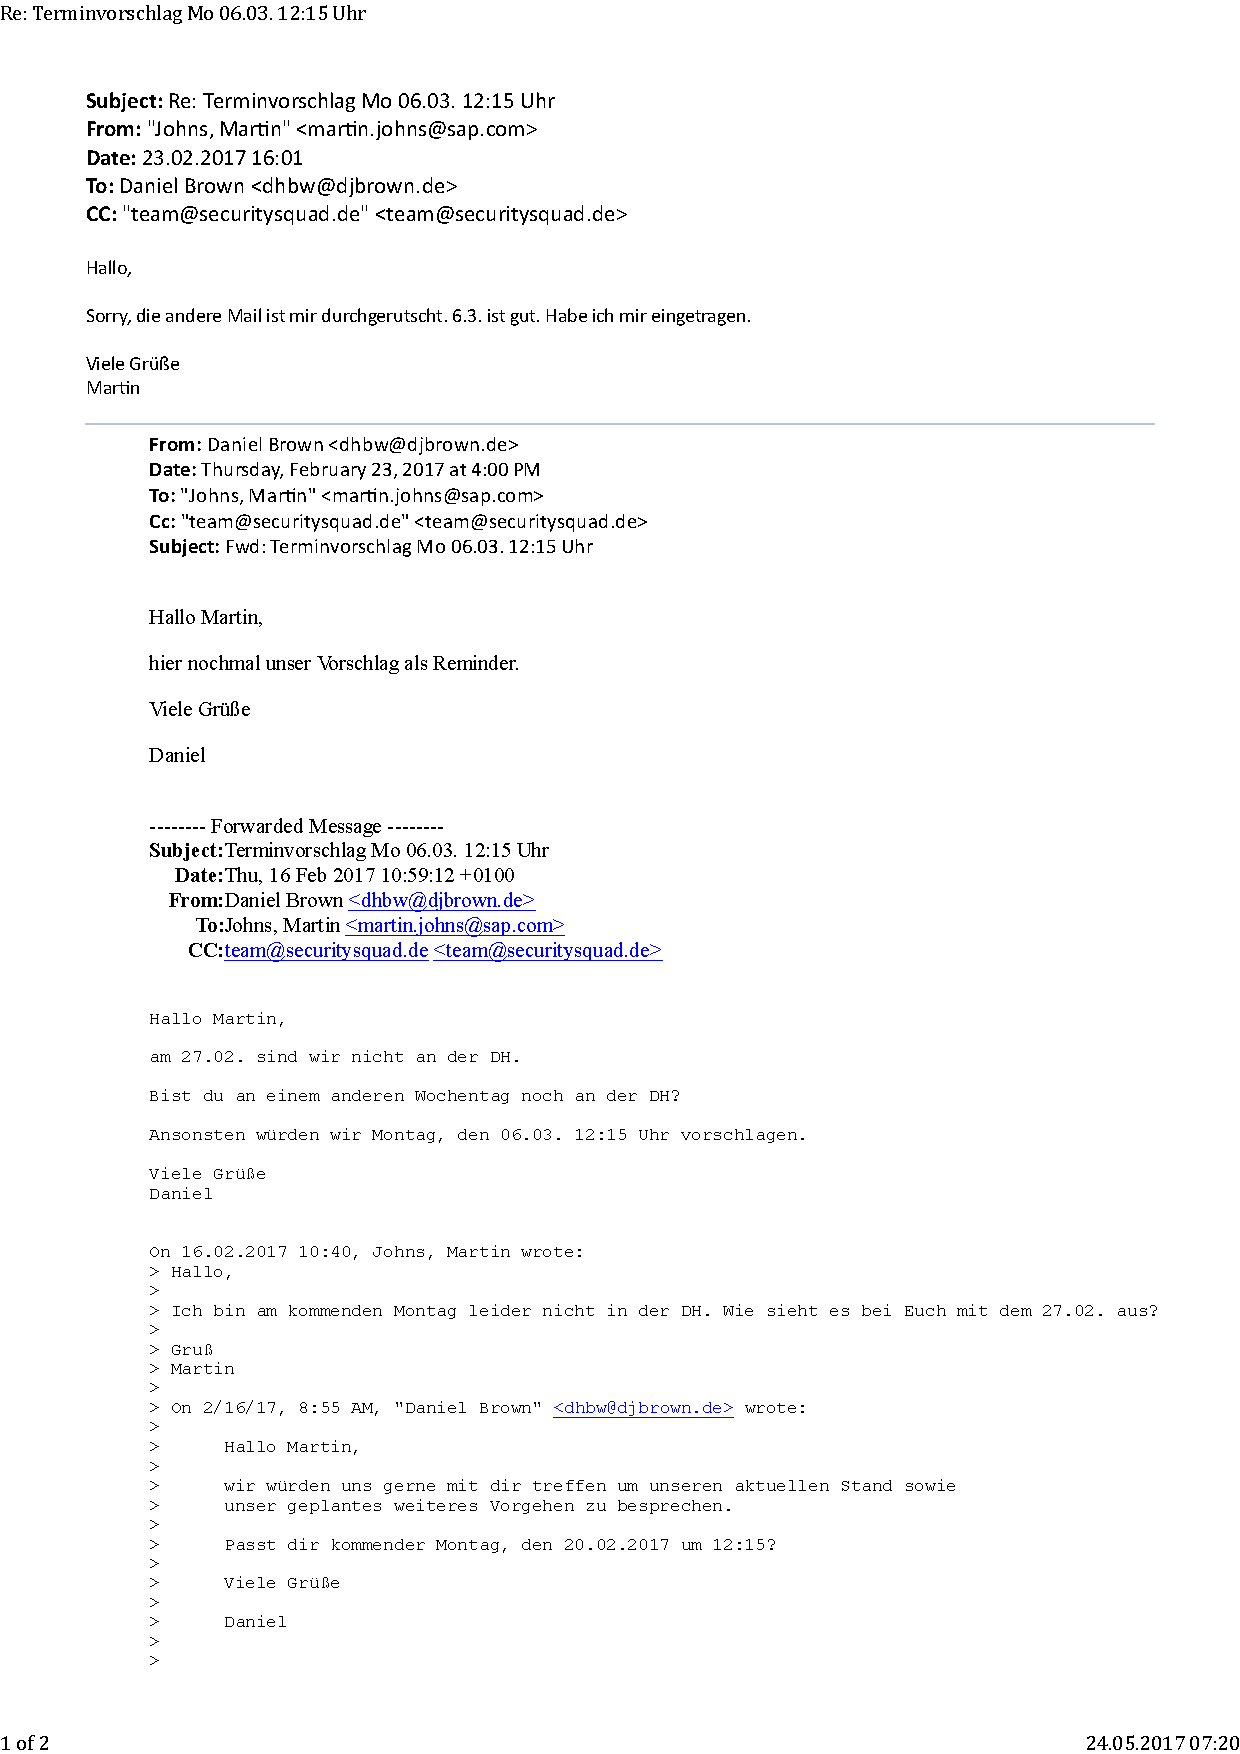
\includepdf[scale=0.8,pages=1,pagecommand=\section{Terminvorschlag Mo 06.03. 12:15 Uhr (16.02. - 06.03.)}\label{mail:termin}]{pdfs/mails/01-terminvorschlag.pdf}


\includepdf[scale=0.8,pages=1,pagecommand=\section{webifier-mail (16.03.)}\label{mail:webifier-mail}]{pdfs/mails/02-webifier-mail.pdf}

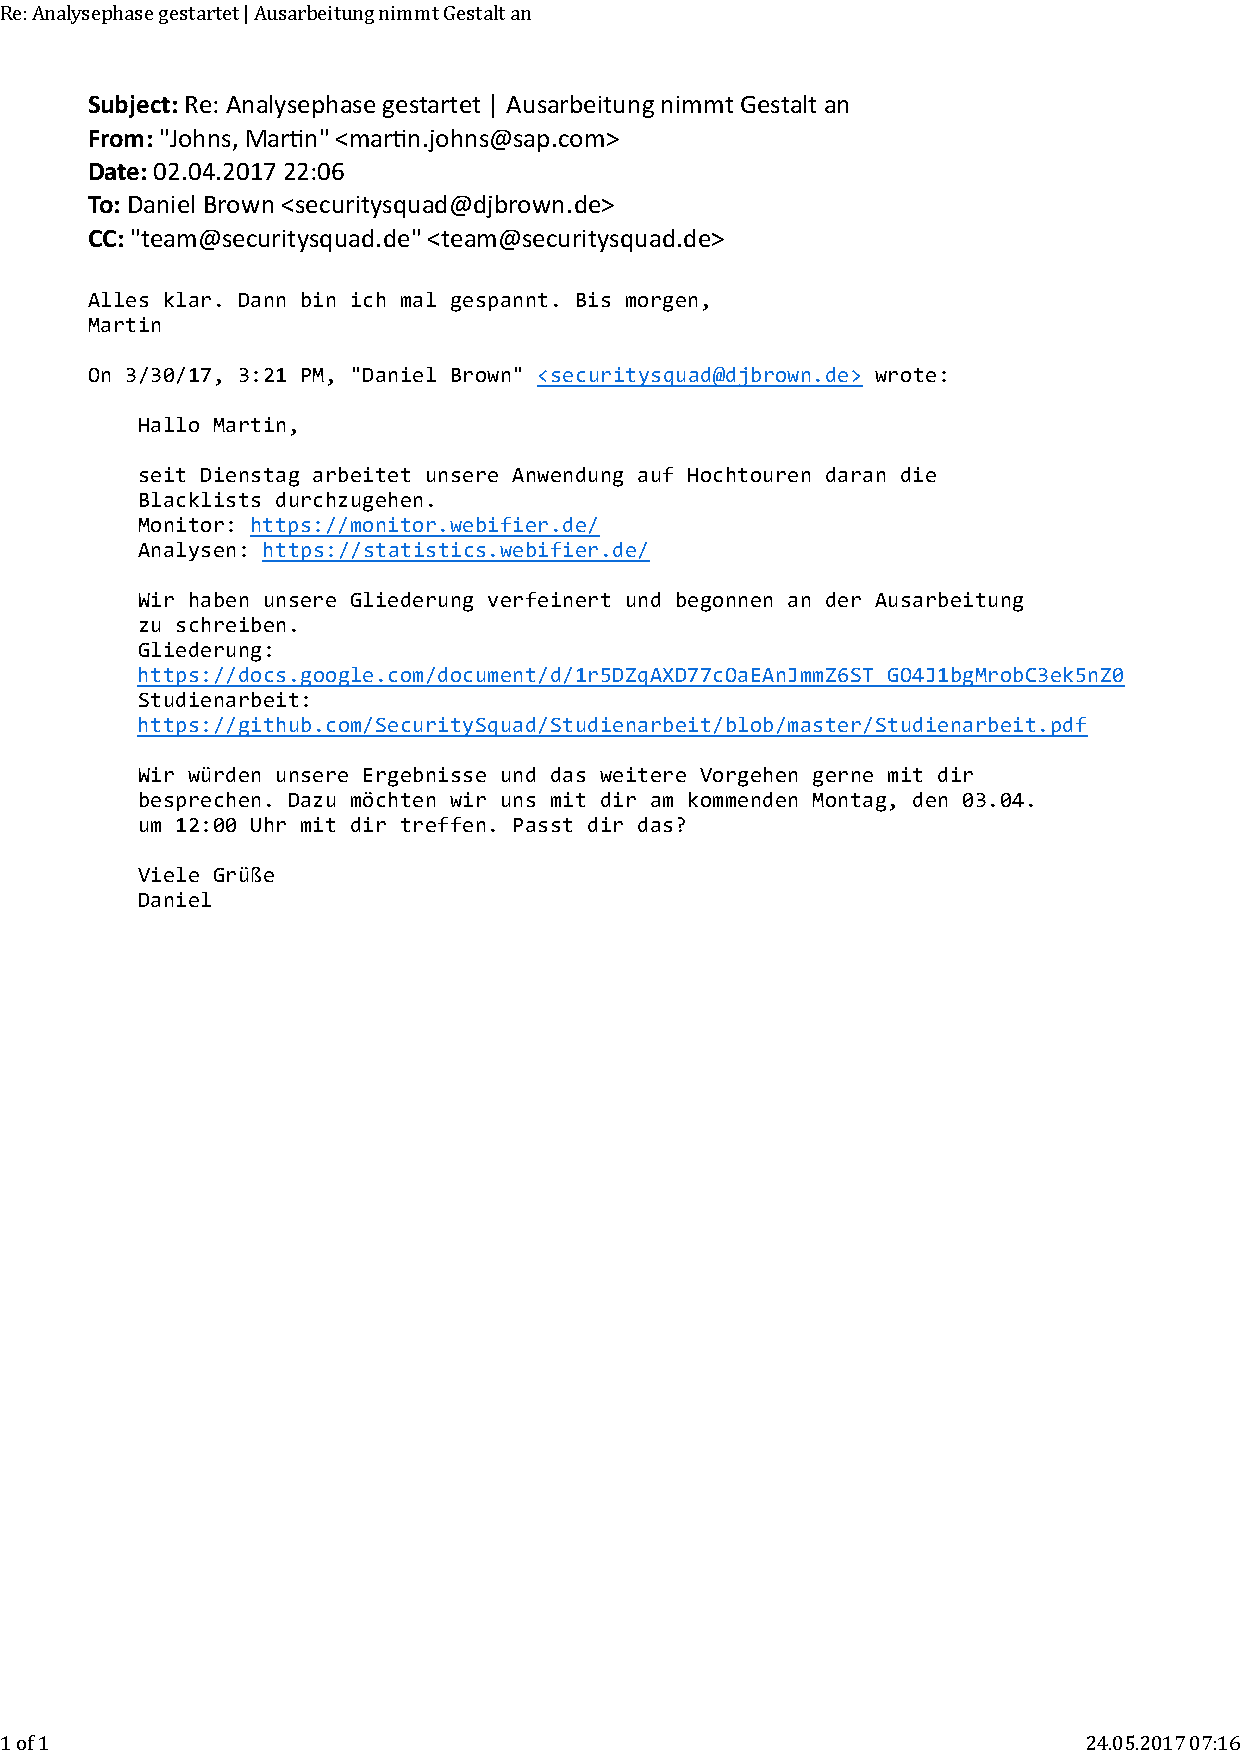
\includepdf[scale=0.8,pages=1,pagecommand=\section{Analysephase gestartet \& Ausarbeitung nimmt Gestalt an (30.03. - 02.04.)}\label{mail:update}]{pdfs/mails/03-update.pdf}


\includepdf[scale=0.8,pages=1,pagecommand=\section{Abuse Hinweis (05.04.)}\label{mail:abuse}]{pdfs/mails/04-abuse.pdf}

\includepdf[pages=2-]{pdfs/mails/04-abuse.pdf}

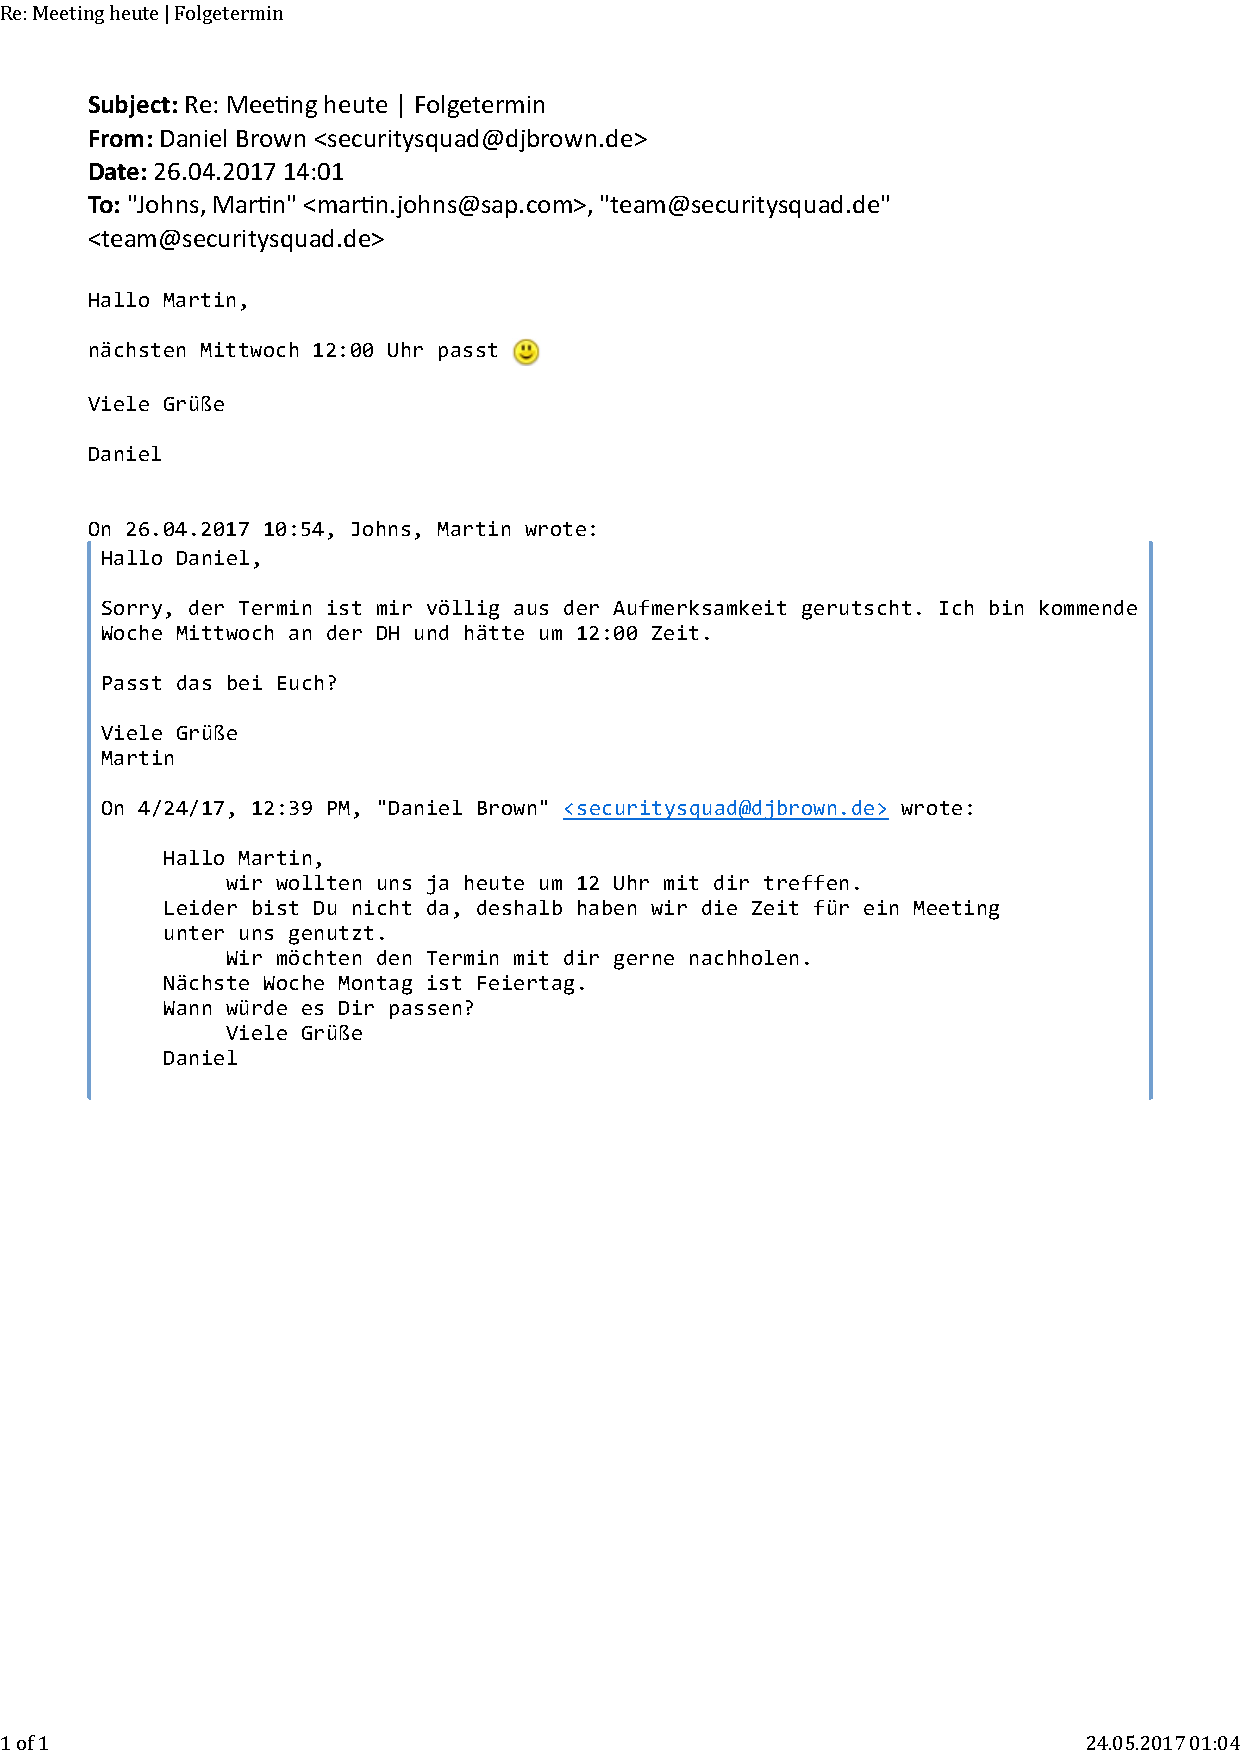
\includepdf[scale=0.8,pages=1,pagecommand=\section{Internes Meeting \& Folgetermin (24.04. - 26.04.)}\label{mail:meeting}]{pdfs/mails/05-meeting.pdf}

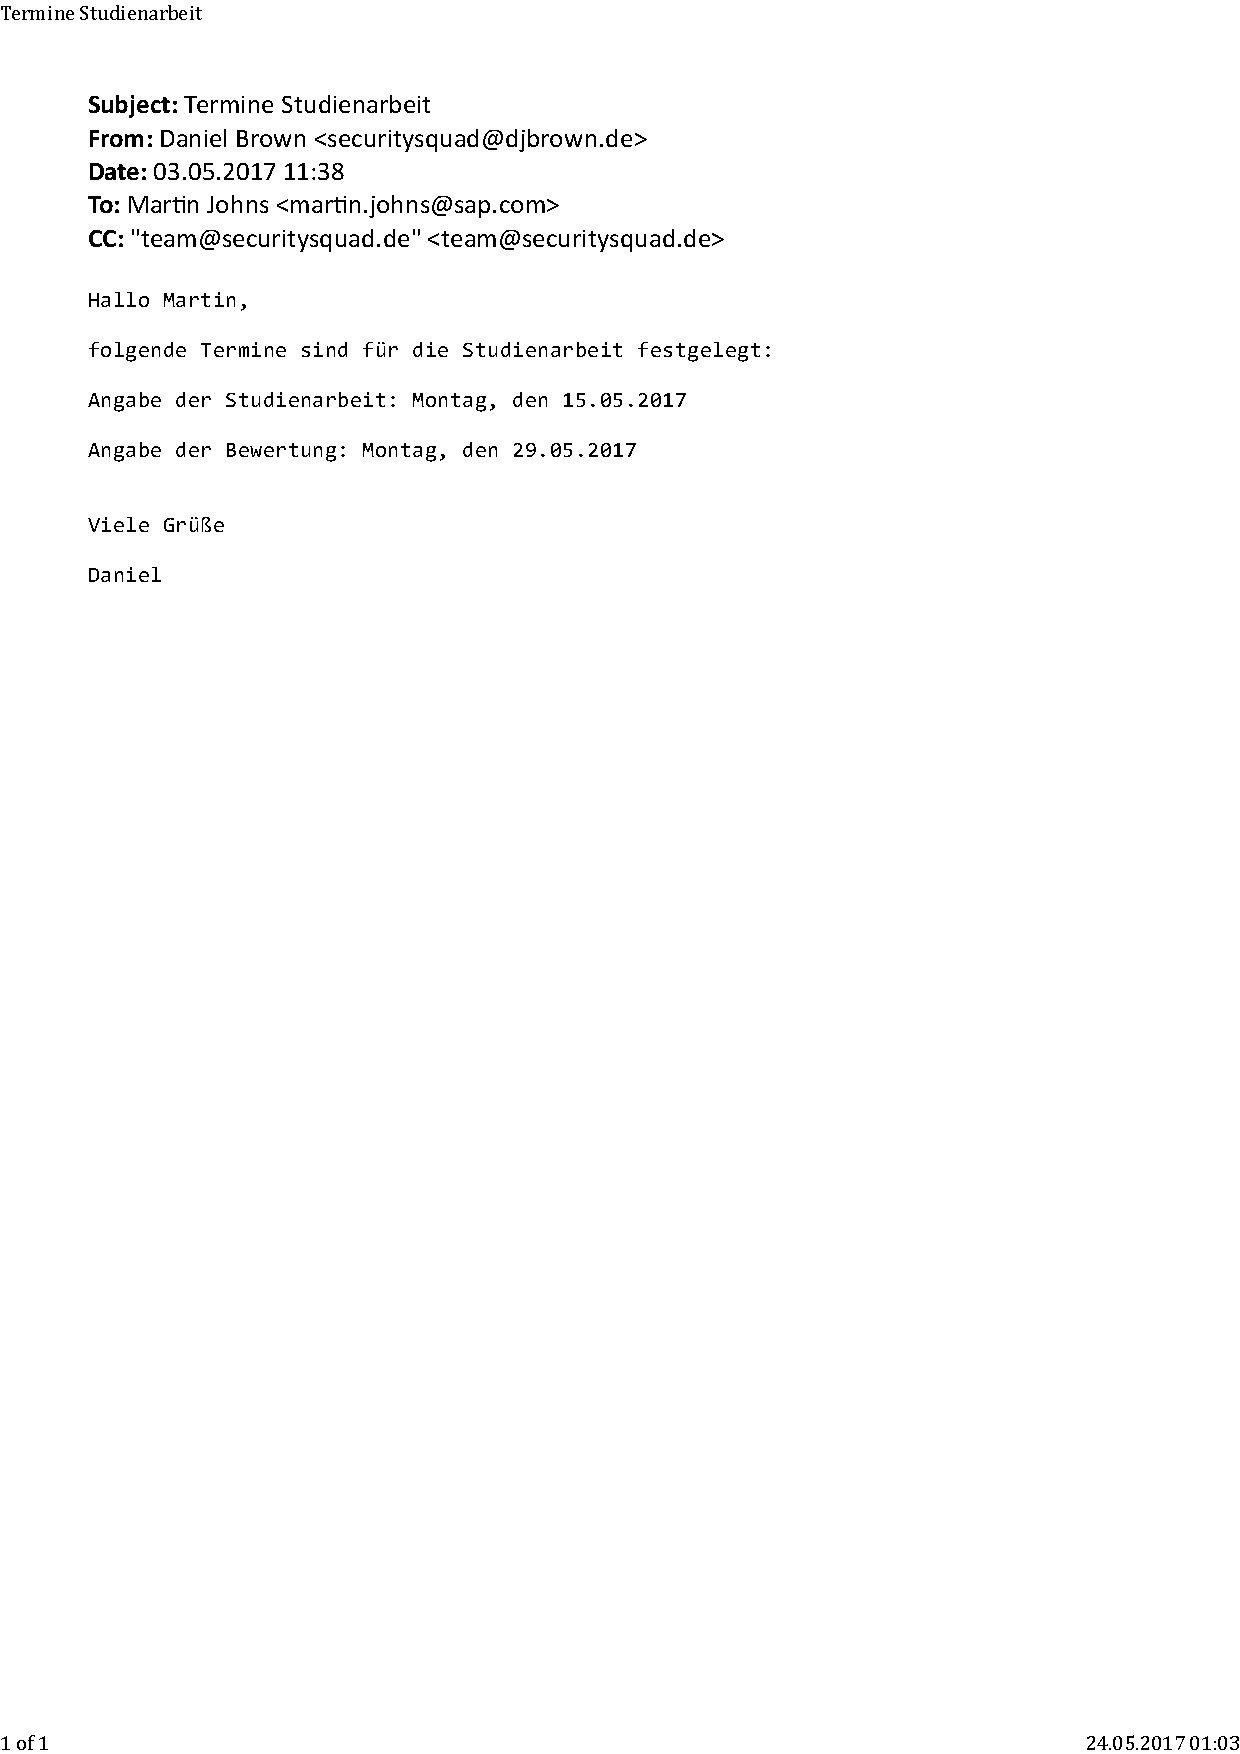
\includepdf[scale=0.8,pages=1,pagecommand=\section{Termine Studienarbeit (24.04. - 03.05.)}\label{mail:termine}]{pdfs/mails/06-termine.pdf}

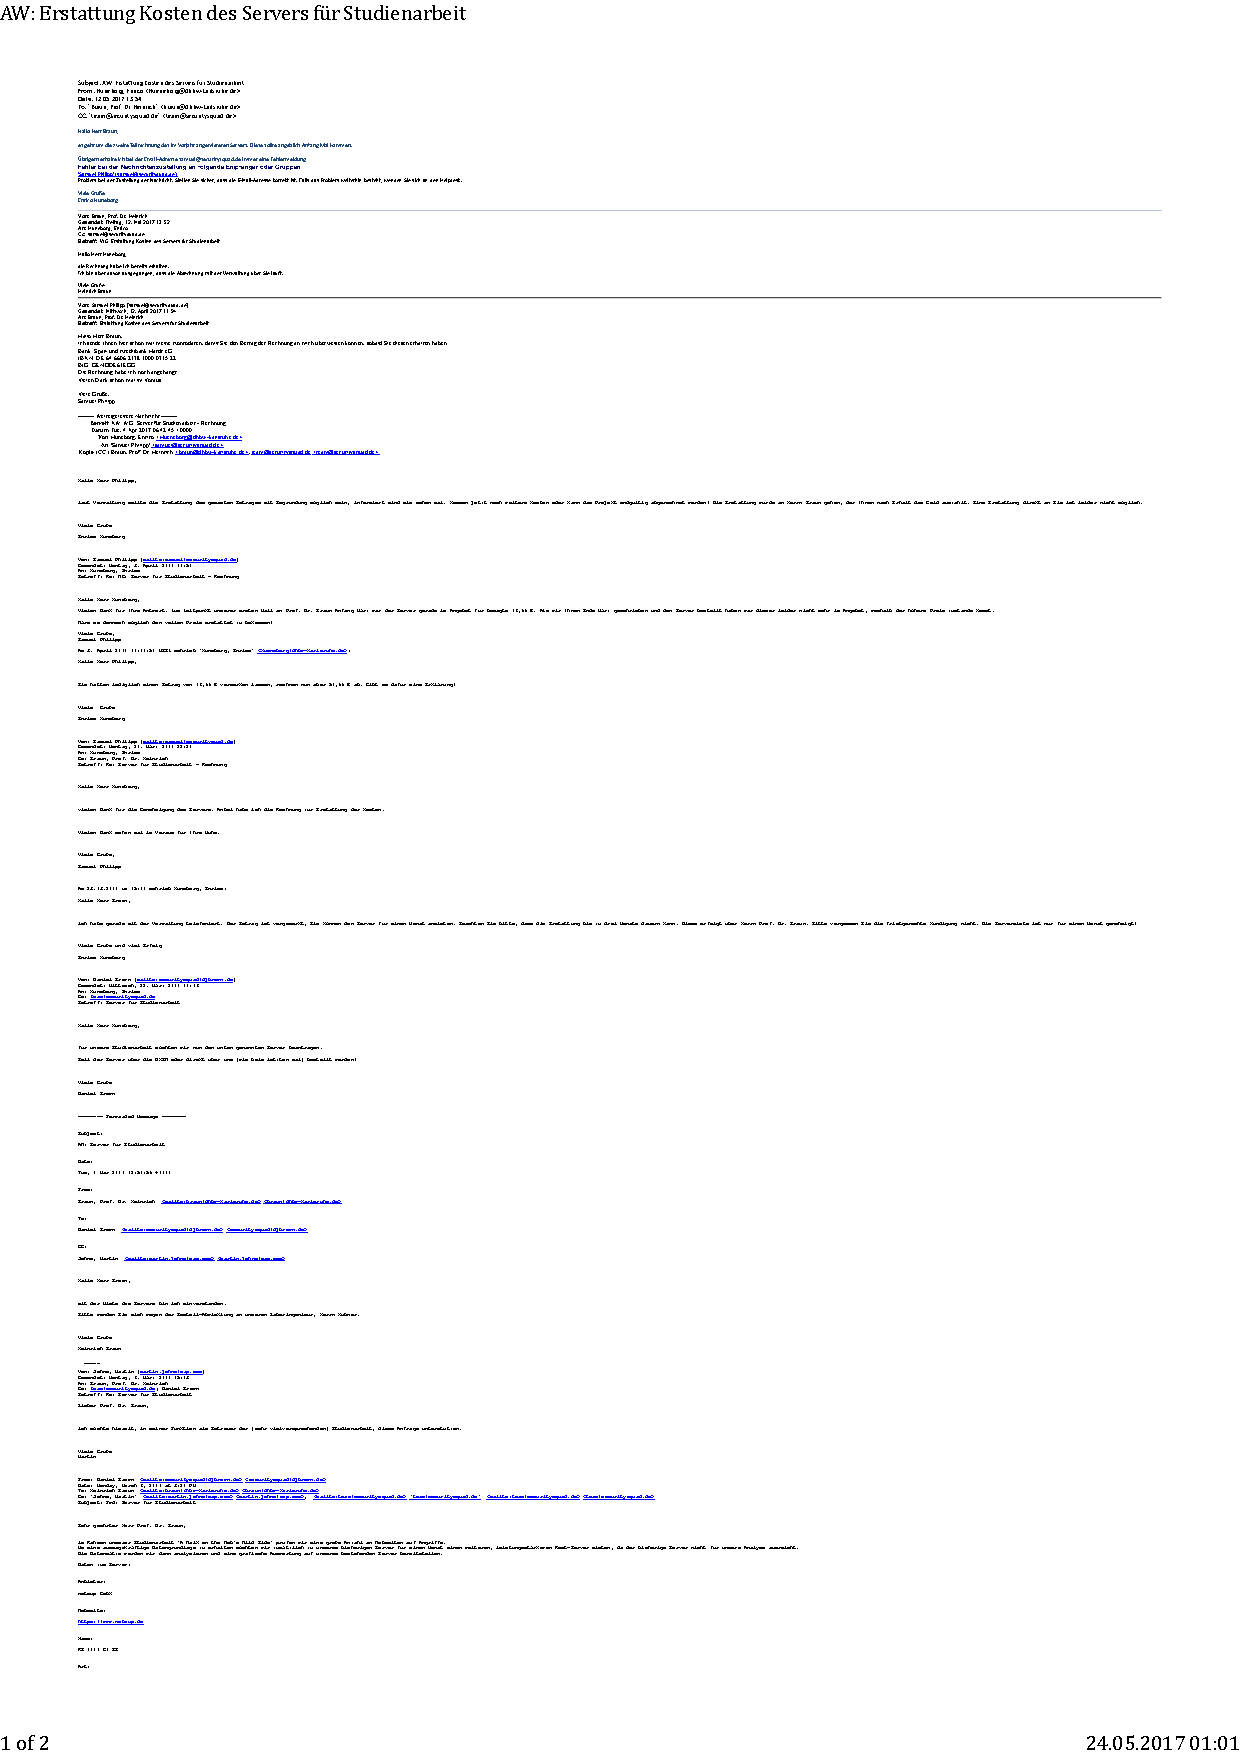
\includepdf[scale=0.8,pages=1,pagecommand=\section{Erstattung Kosten des Servers für Studienarbeit (24.04. - 12.05.)}\label{mail:erstattung}]{pdfs/mails/07-erstattung.pdf}
\includepdf[pages=2-]{pdfs/mails/07-erstattung.pdf}

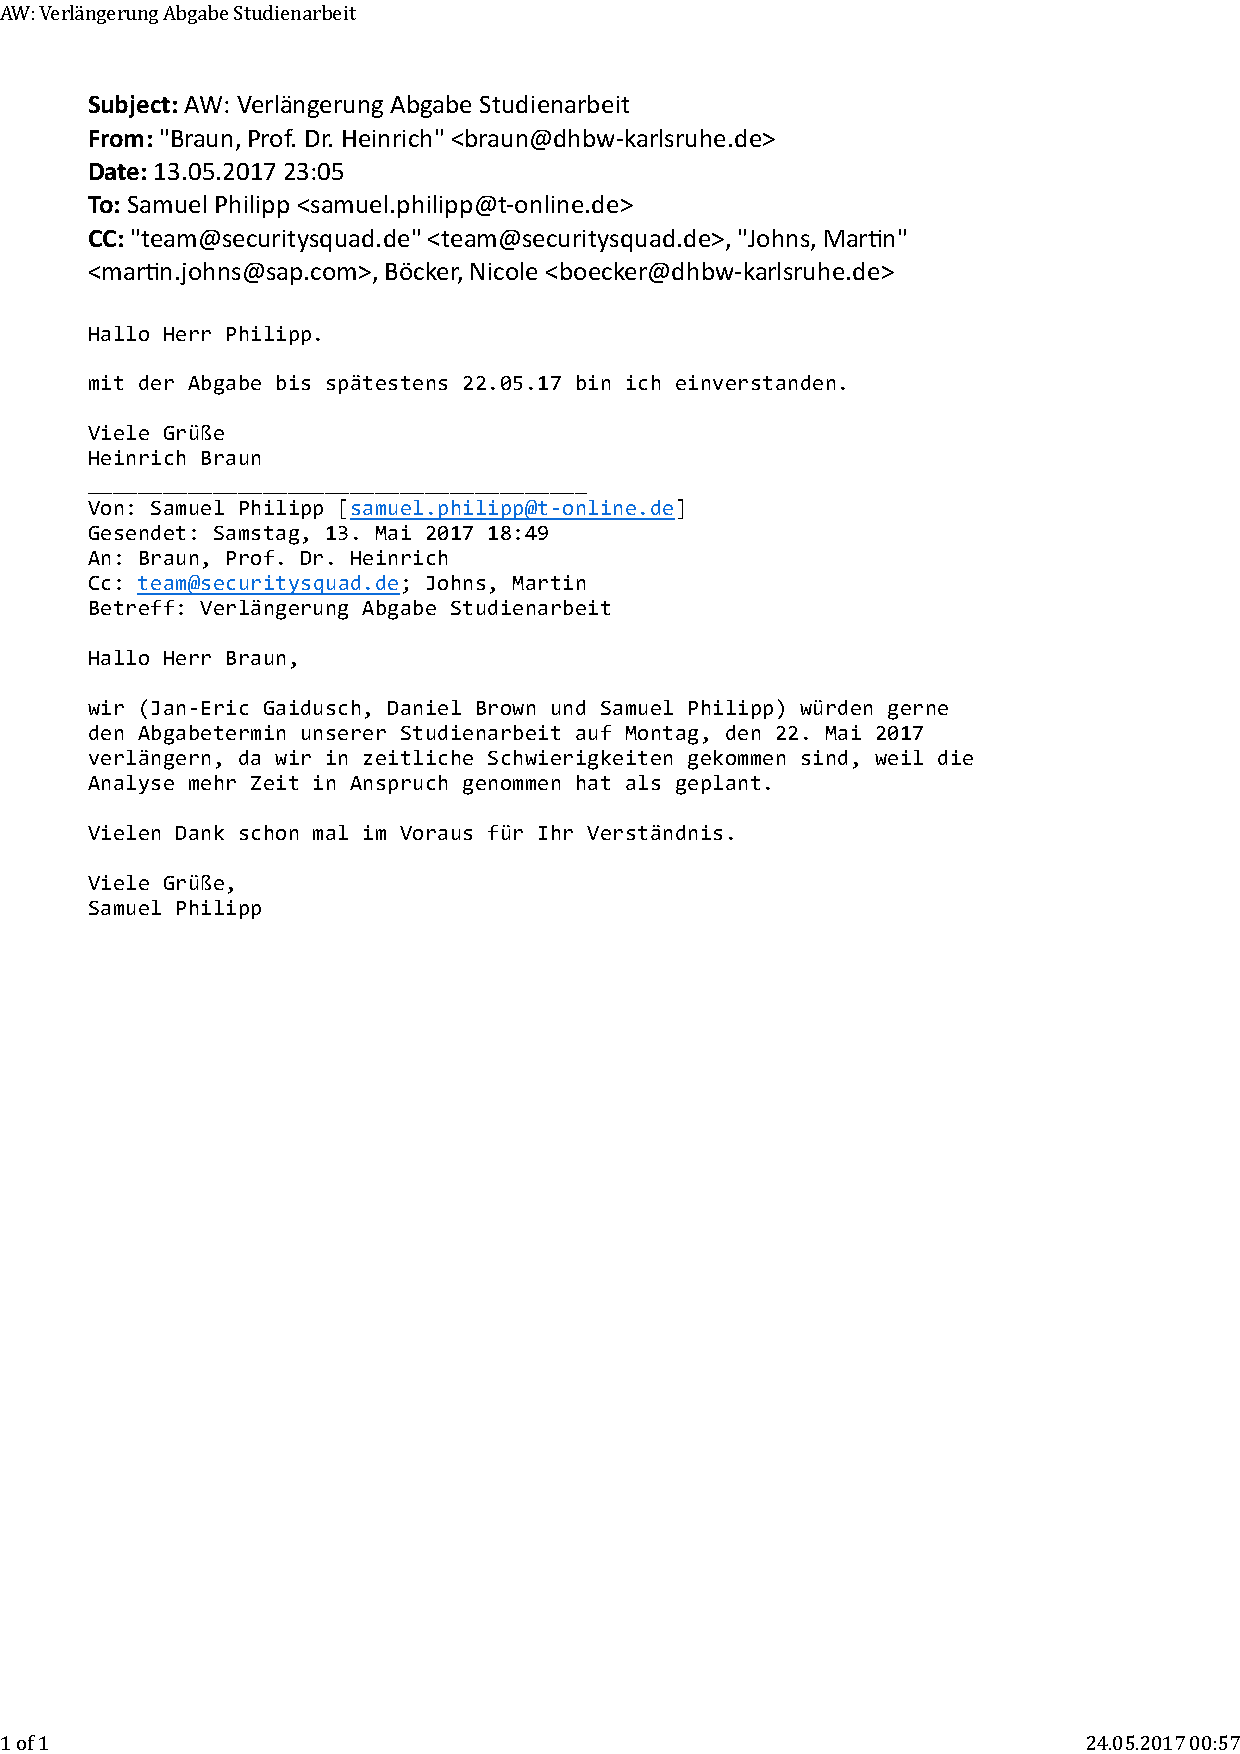
\includepdf[scale=0.8,pages=1,pagecommand=\section{Verlängerung Abgabe Studienarbeit (13.05.)}\label{mail:verlängerung}]{pdfs/mails/08-verlaengerung.pdf}


\includepdf[scale=0.8,pages=1,pagecommand=\section{Korrekturlesen Studienarbeit (16.05. - 17.05.)}\label{mail:korrektur}]{pdfs/mails/09-korrektur.pdf}

\includepdf[pages=2-]{pdfs/mails/09-korrektur.pdf}

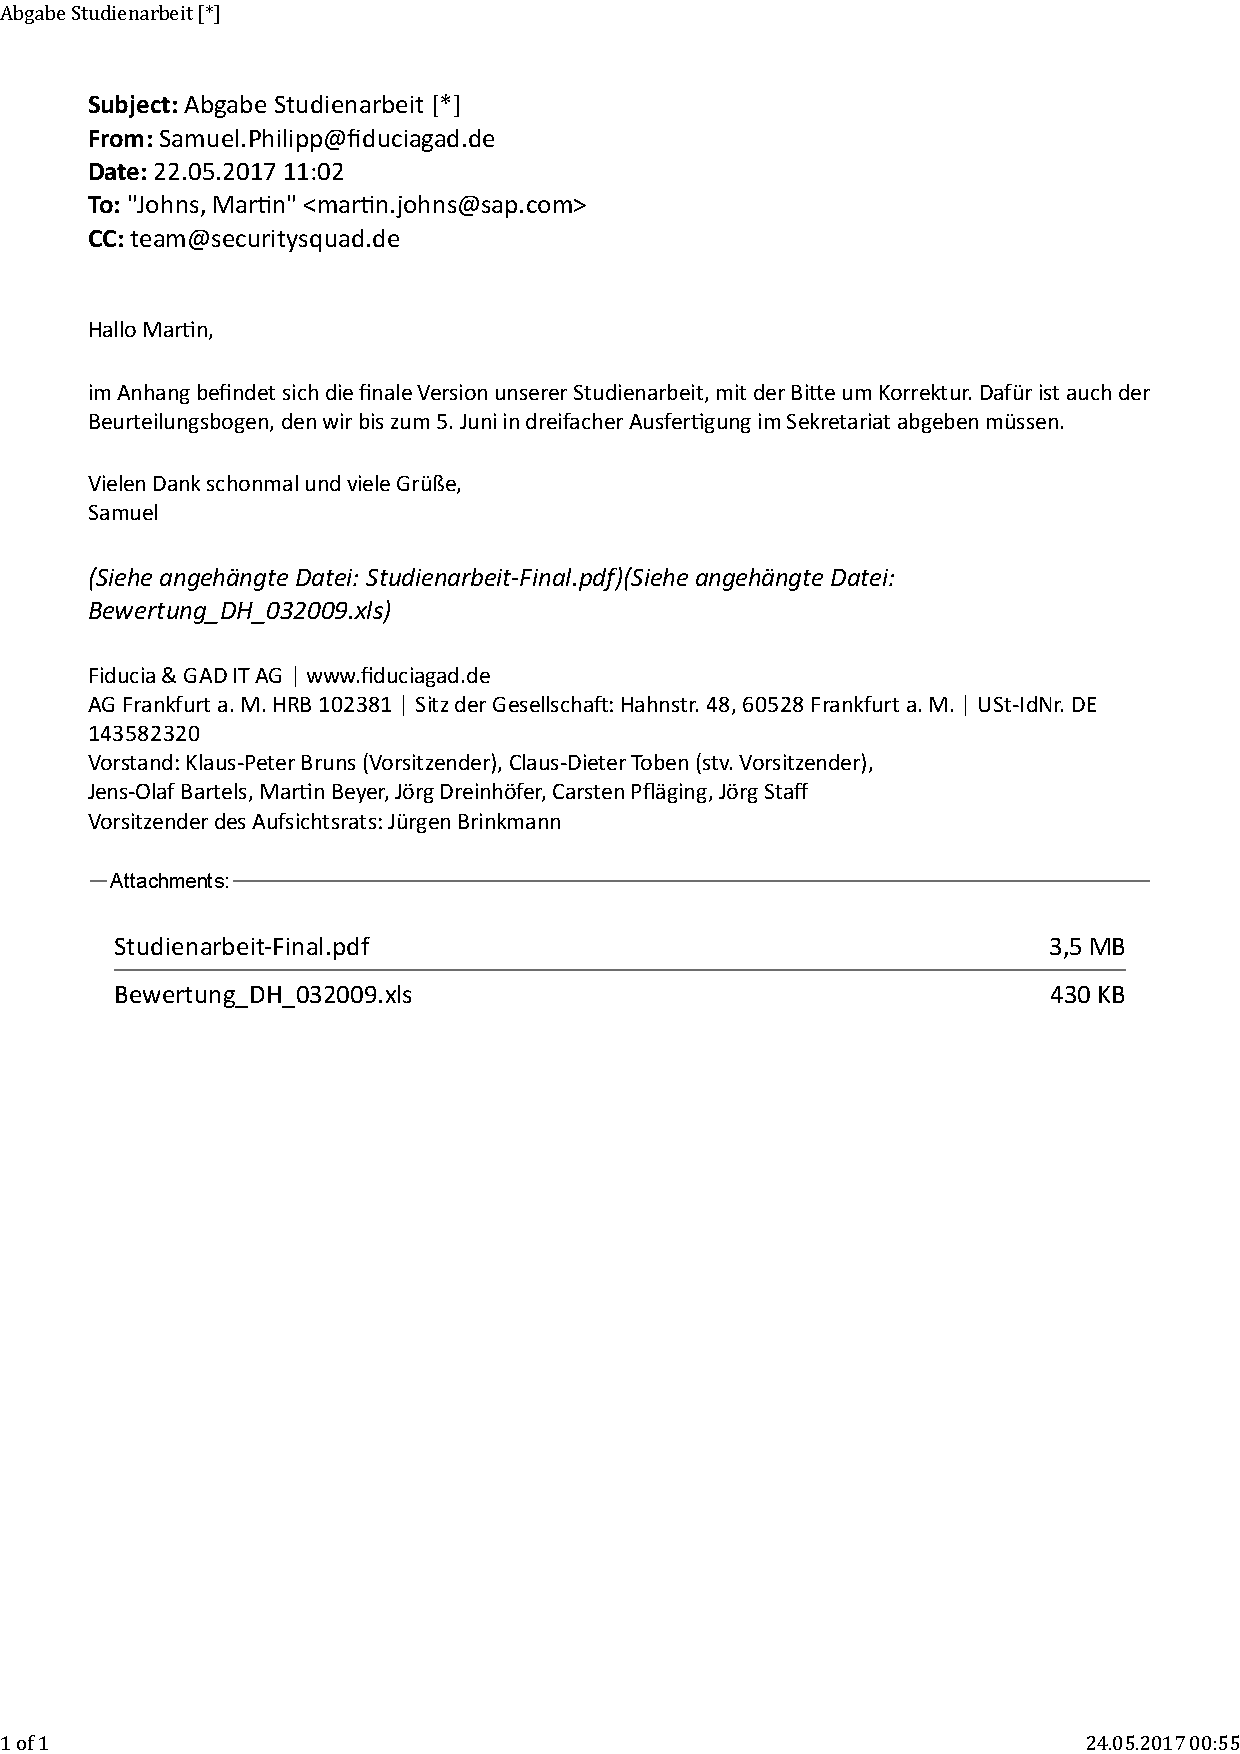
\includepdf[scale=0.8,pages=1,pagecommand=\section{Abgabe Studienarbeit (22.2.05.)}\label{mail:abgabe}]{pdfs/mails/10-abgabe.pdf}


\chapter{Protokolle}


\includepdf[scale=0.8,pages=1,pagecommand=\section{Dokumentation der Meetings}\label{pdf:meetings}]{pdfs/meetings.pdf}

\includepdf[pages=2-]{pdfs/meetings.pdf}


\end{document}
